\chapter{Desenvolvimento do projeto}
\label{chap:metod}
Nesta seção será descrito o procedimento utilizado para construção de cada um dos desafios.

\section{Webots}
O robô utilizado foi o Pionner o qual usa seus 16 sensores de distância pré-instalados para obter informações do mundo em todas as direções 
e um sensor adcional:o sensor de luminosidade que rastreia a irradiância local e envia um sinal para o robô quando ele lê mais de 750 W / m2, 
o que significa que está perto o suficiente da luminária de chão para disparar o STOP.

\subsection{controle}
A navegação do robô pelo mapa é baseada em uma máquina de 4 estados que determina se ele deve se mover para frente,
virar à esquerda, direita ou parar quando atingir seu objetivo final.

Assim, a divisão foi feita em quatro casos, são eles:
\begin{itemize}
    \item FORWARD: Anda para frente e se houver algum obstáculo à frente ele começa a tomar a decisão de virar em qualquer direção para evitá-lo.
    \item ESQUERDA: Vire à esquerda até que a detecção de objetos não seja mais possível;
    \item DIREITA: Vire à direita até que a detecção de objetos não seja mais possível;
    \item STOP: Quando o sensor de luz detecta a quantidade de luminosidade configurada (neste caso 750 W / m2), o robô deve parar.
\end{itemize}
Todos os sensores de distância coletam dados do ambiente que determinam se o robô deve se mover para frente ou para os lados.
\section{Turtlesim}
Para que o desafio seja cumprido é necessário rodar o roscore e o nó para que a janela da turtle apareça na tela.

\begin{figure} [h!]	
    \centering
    \caption{inicializando o ros}
    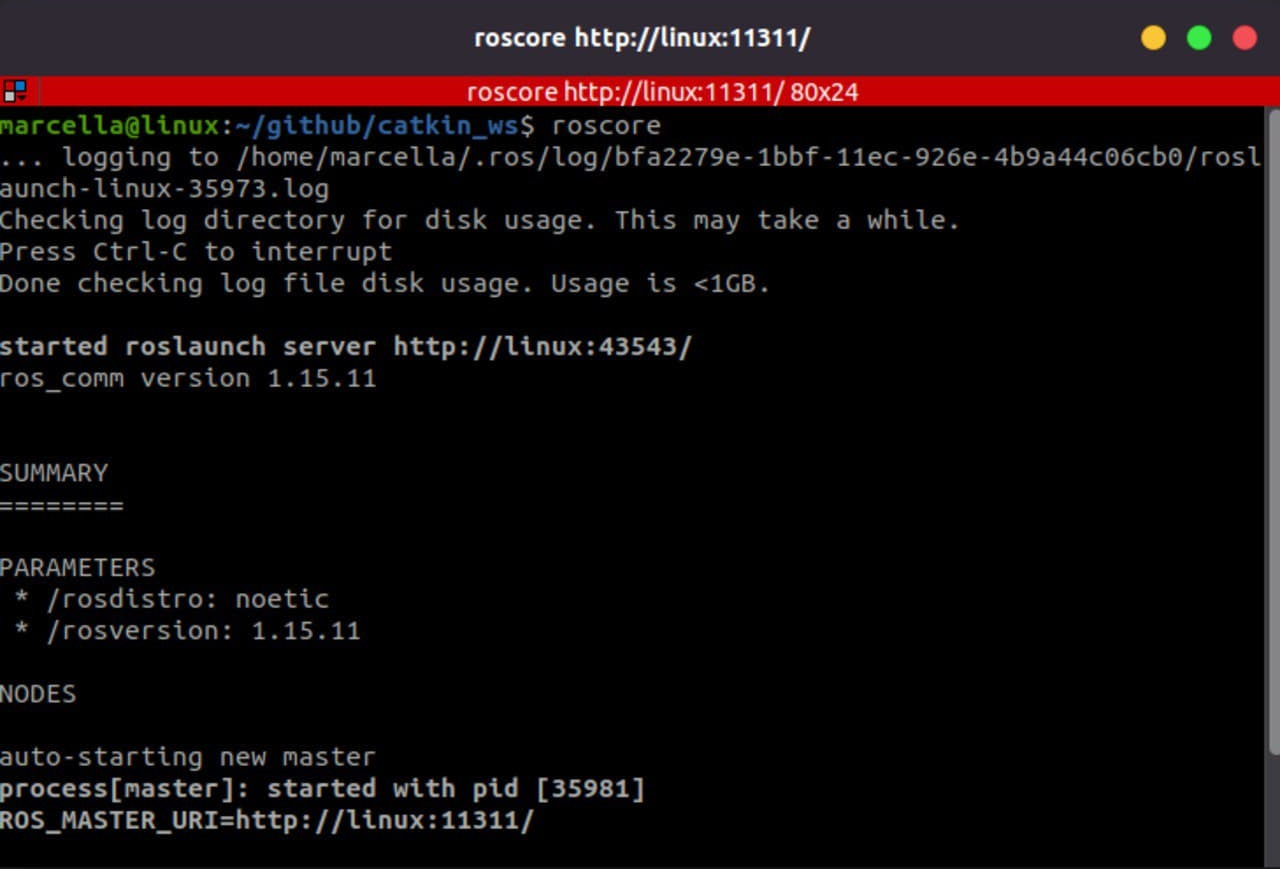
\includegraphics[width=0.5\textwidth]{roscore.jpg}
    \caption*{Fonte: Autoria própria.}
    \label{fig:roscore}
\end{figure}

\begin{figure} [h!]	
    \centering
    \caption{ Rodando o nó do turtlesim}
    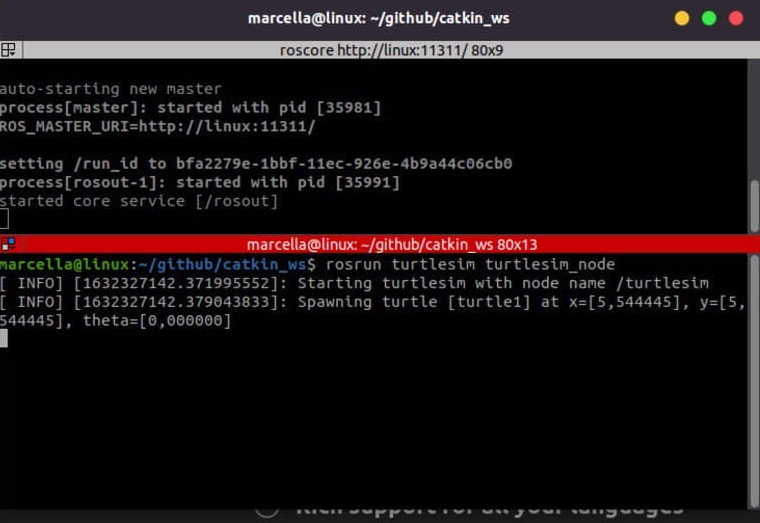
\includegraphics[width=0.5\textwidth]{rosrum.jpg}
    \caption*{Fonte: Autoria própria.}
    \label{fig:rosrum}
\end{figure}
por fim executa-se o arquivo .py quue foi a liguagem escolhida para completar este desafio, como mostra a figura abaixo.
\begin{figure} [h!]	
    \centering
    \caption{ Executando arquivo}
    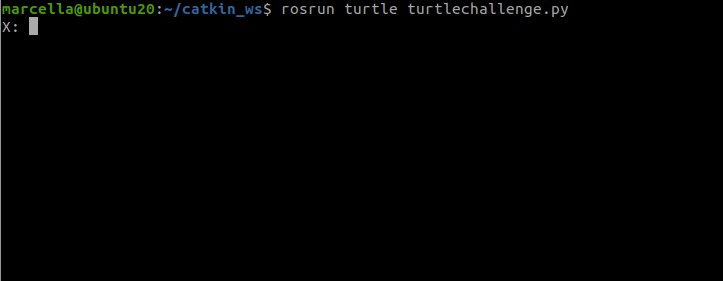
\includegraphics[width=0.5\textwidth]{xey.jpeg}
    \caption*{Fonte: Autoria própria.}
    \label{fig:excute.py}
\end{figure}
É posto as coordenadas x e y no caso do exemplo do desafio é 1 e 1 e a tartaruga deve ir até essa coordenada quando o erro for no máximo 0.1.
\section{Husky}
\subsection{Move Base}
Após toda a configuração e instalação dos pacotes do Husky encontrado no repositório https://github.com/husky/husky, foi executado o nó move-base no qual será enviado um comando para o robô Husky que tentará atingir a posição enviada desviando dos obstáculos e caso entre em alguma posição em que se esteja travado executa comportamentos de recuperação para continuar o trajeto enviado.

Para a execução do nó move-base é necessário trés comandos o primeiro inicia o ambiente de simulação o gazebo, o segundo o visualizador rviz e o terceiro a demonstração move-base.
\begin{figure} [h!]	
    \centering
    \caption{Comandos move base}
    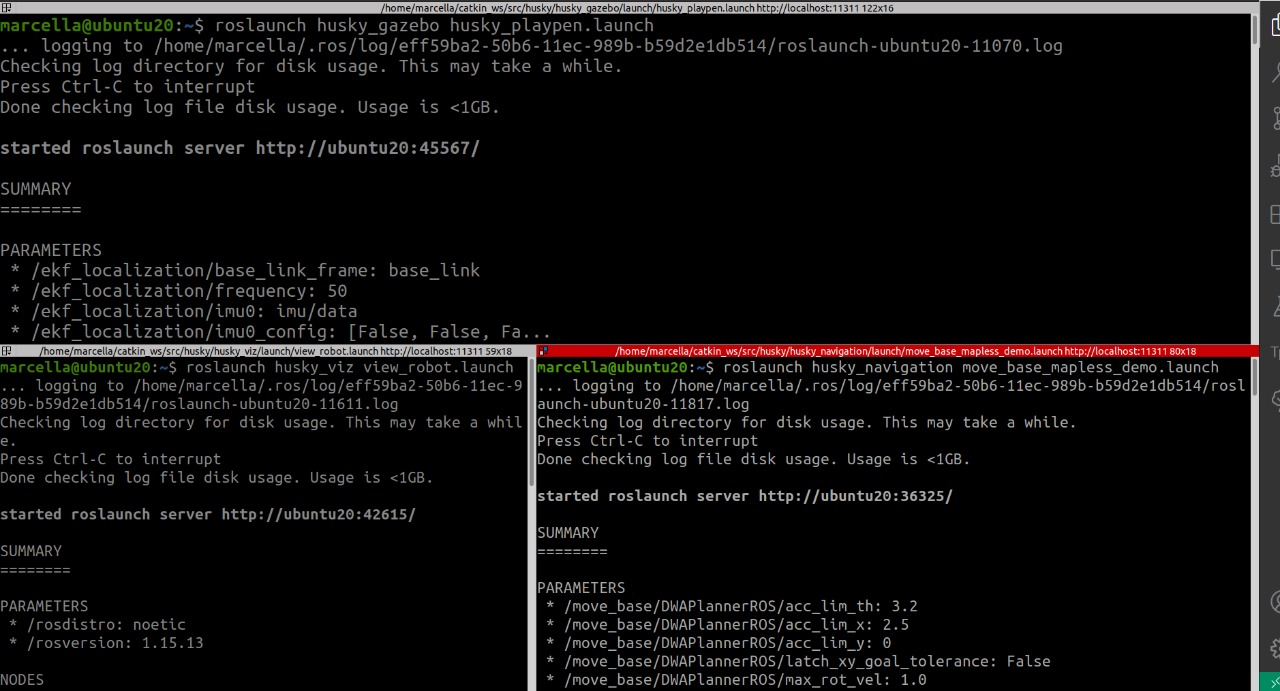
\includegraphics[width=0.9\textwidth]{comandosmb.jpeg}
    \caption*{Fonte: Autoria própria.}
    \label{fig:movebase}
\end{figure}
\subsection{AMCL}
O Tutorial amcl do Husky mostra como é usado o move-base com o sendo assim, amcl obtém um mapa baseado em laser que precisa ser ativado no description do robô encontrado no próprio repositório após a ativação o laser faz varreduras e transforma em mensagens que geram estimativas de posição.
\begin{figure} [h!]	
    \centering
    \caption{Comandos amcl}
    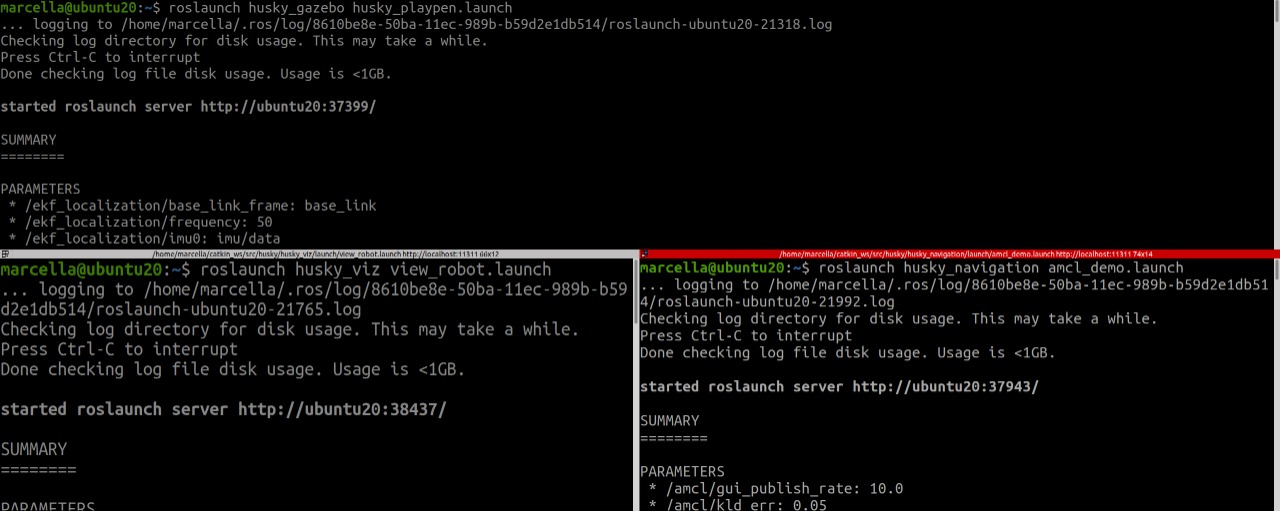
\includegraphics[width=0.9\textwidth]{comandosamcl.jpeg}
    \caption*{Fonte: Autoria própria.}
    \label{fig:amcl}
\end{figure} 
\subsection{gmapping}
Após a execução do nó slam-gmapping será levado para o tópico sensor-msgs/LaserScan mensagens e constrói um mapa a partir dos dados de laser e posições coletados pelo husky.
\begin{figure} [h!]	
    \centering
    \caption{Comandos gmapping}
    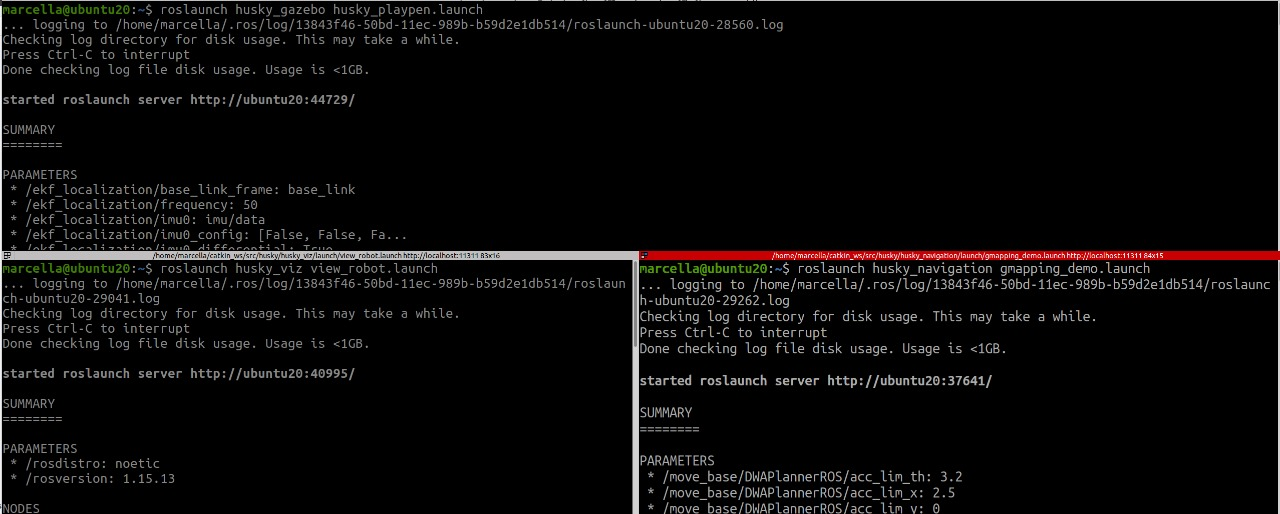
\includegraphics[width=0.9\textwidth]{comandogm.jpeg}
    \caption*{Fonte: Autoria própria.}
    \label{fig:gmapping}
\end{figure}
\subsection{Frontier-exploration}
O Frontier-exploration pacote fornece um costmap-2d que fornece uma implementação de um mapa de custo 2D que leva em dados de sensor do mundo, constrói uma grade de ocupação 2D ou 3D dos dados, e actionlib cliente que fornece uma interface padronizada com tarefas preemptivas
\begin{figure} [h!]	
    \centering
    \caption{Comandos frontier-exploration }
    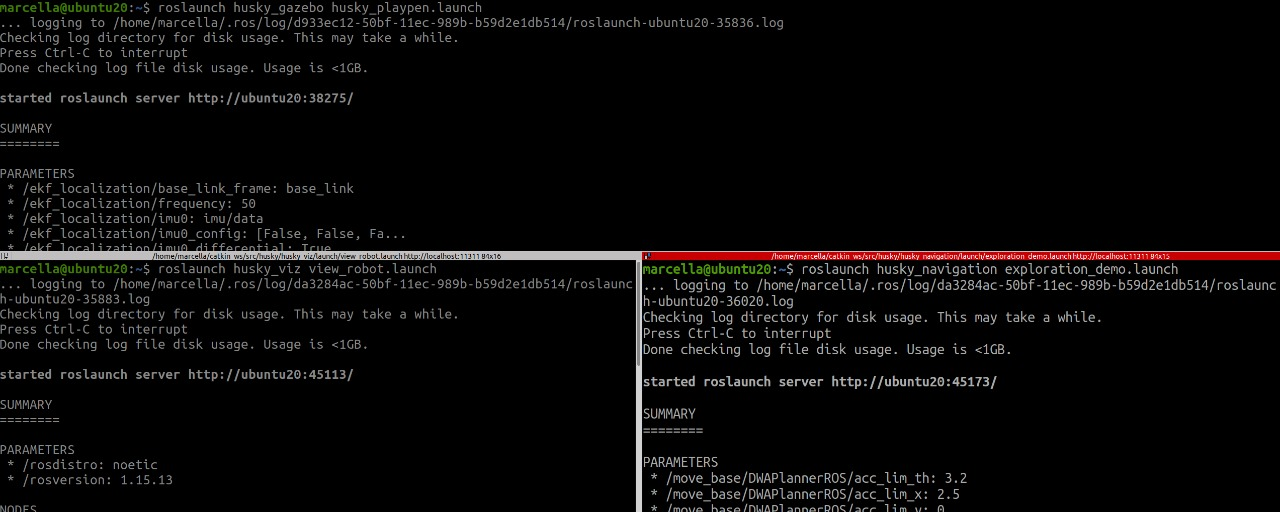
\includegraphics[width=0.9\textwidth]{comandosf.jpeg}
    \caption*{Fonte: Autoria própria.}
    \label{fig:frontier-exploration}
\end{figure}
\section{CPP}
\section{Python}
% %--------- NEW SECTION ----------------------
% \section{Interface do Usuário}
% \label{sec:ui}
% \lipsum[1]

% %--------- NEW SECTION ----------------------
% \section{Simulação do sistema}
% \label{sec:sim}
% \lipsum[2-4]

